\ifdefined\USERMANUAL
  \newcommand{\doctype}{USER'S MANUAL}
\else
  \newcommand{\doctype}{REFERENCE CARDS}
\fi

\maketitlepage{TAIPO}{MIDI Extender}{TAIPO_SILVER_cutout_small_2}{\doctype}

\newpage
\tableofcontents
\newpage
\part{Overview}
\newpage
\section{Overview}\label{section:installation}
\subsection{Overview}
\paragraph*{}
The \textbf{TAIPO} MIDI Extender enables seamless connection of The Centre to external equipment, including computers, using a standard MIDI TRS Type B cable.
\subsection{What's in the Box}
\paragraph*{}
The \textbf{TAIPO} package includes the following accessories:
\begin{enumerate}
  \item \textbf{TAIPO} Eurorack module
  \item Standard Eurorack power cable (10-pin to 16-pin)
  \item MIDI-EX link cable for connecting to \textbf{The Centre}
\end{enumerate}

\newpage
\part{Installation}
\newpage
\section{Installation}
\subsection{Installation Steps}
\paragraph*{}
Installing the \textbf{TAIPO} follows the standard procedure for installing any Eurorack module in your case.

\begin{figure}[h]
  \centering
  \includegraphics[height=0.5\linewidth]{taipo_the_centre_cable_install.jpg}
  \includegraphics[height=0.5\linewidth]{taipo_cable_install.jpg}
  \caption{Cable installation on both ends}
  \label{fig:midsinglenote}
\end{figure}

\subsection{Important Installation Notes}
\paragraph*{}
Ensure correct cable orientation during installation. The color order on The Centre side should be \textbf{BLACK, RED, YELLOW, GREEN} from the top, while on the TAIPO side, it should be \textbf{GREEN, YELLOW, RED, BLACK}.
\newline$\blacksquare$ \textbf{Important}: On The Centre side, connect to the MIDI-EX connector as shown in the figure above. The second connector is designated for linking The Centre’s MIDI output to TWINS.

\newpage
\part{MIDI}
\newpage
\section{MIDI Cable Types}
\subsection{TAIPO Cable Type}
\paragraph*{}
The \textbf{TAIPO} utilizes a MIDI 3.5mm TRS (Tip-Ring-Sleeve) Cable Type B. See: \underline{\nameref{section:cabletypeb}}
\subsection{About MIDI Signal}
\paragraph*{}
The MIDI signal is transmitted over a MIDI cable using the RS-232 protocol at a non-standard speed of 31,250 baud (bits per second). MIDI connections are directional, meaning the internal pin configuration within the cable is critical as the current flows in one direction. While standard MIDI DIN cables pose no issues, 3.5mm TRS cables can vary due to the lack of an initial universal standard, resulting in different wiring configurations. Several standards have since emerged.
\newline$\blacksquare$ \textbf{Note}: Different TRS standards are not interchangeable or compatible. To connect devices with differing TRS standards, a compatible cable must be used.
\subsection{DIN Connector}
The standard MIDI cable employs a 5-pin DIN connector for reliable connectivity.
\subsection{TRS Connector Types}
\subsubsection{Type A Connector}
Type A TRS defines the \textbf{TIP} of the 3.5mm jack as the \textit{\textbf{source}} and the \textbf{RING} as the \textit{\textbf{sink}}.
\newline
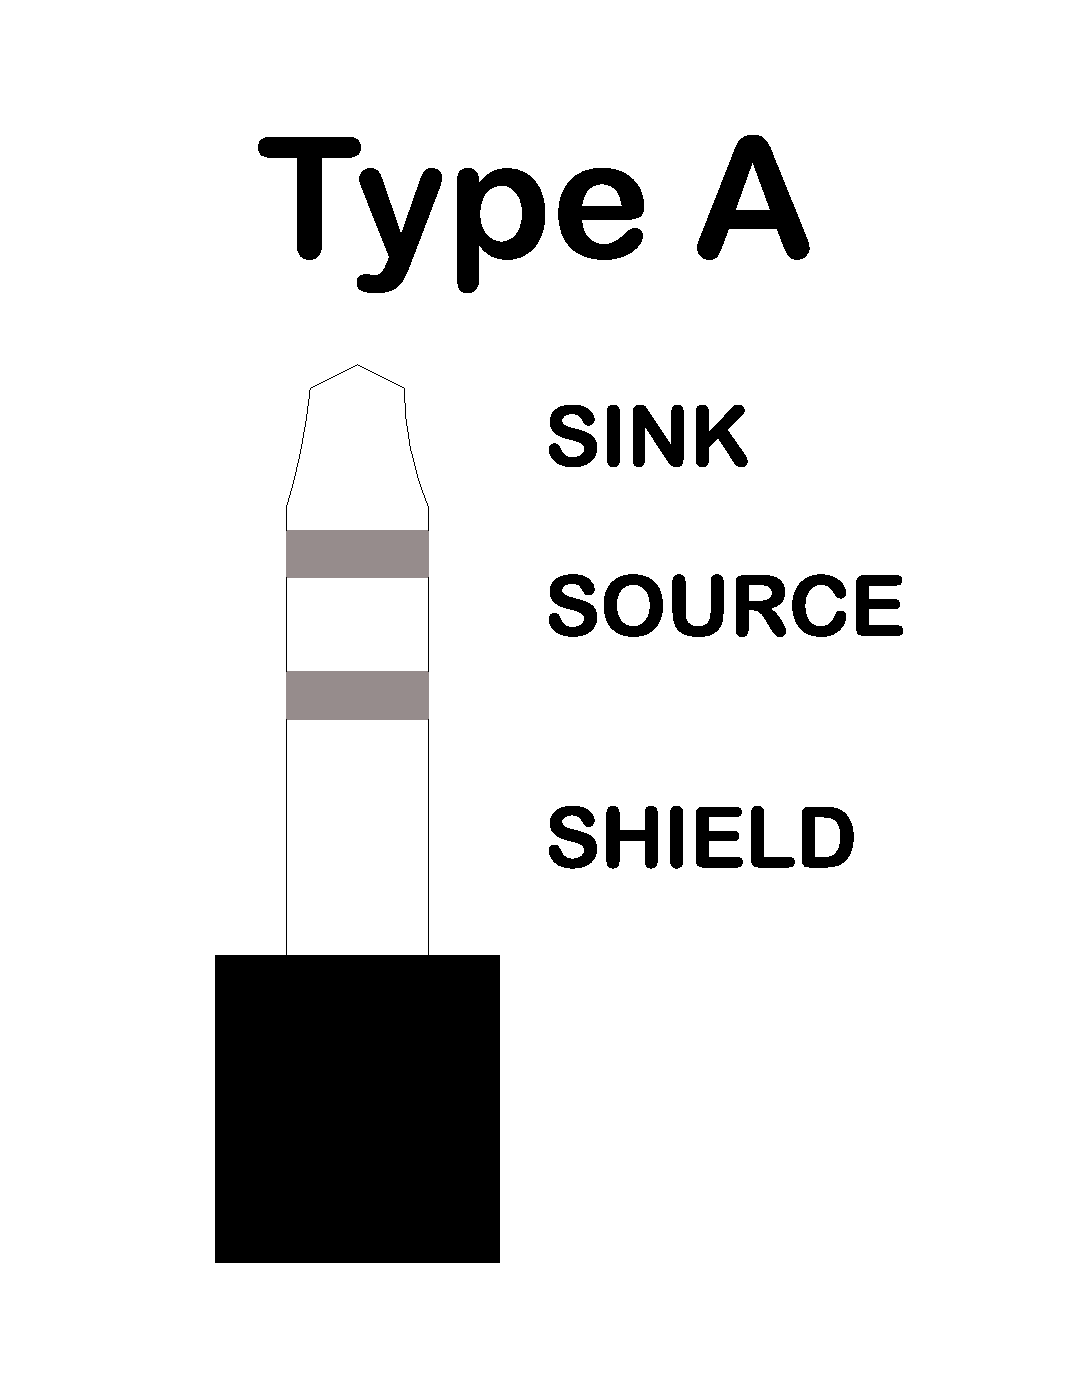
\includegraphics[height=0.3\linewidth]{midi_trs_type_a.eps}
\newline$\bigstar$ Brands using Type A: Korg, Akai
\subsubsection{Type B Connector}\label{section:cabletypeb}
Type B TRS defines the \textbf{TIP} of the 3.5mm jack as the \textit{\textbf{sink}} and the \textbf{RING} as the \textit{\textbf{source}}.
\newline$\blacksquare$ Type B is widely adopted in the Eurorack modular community.
\newline
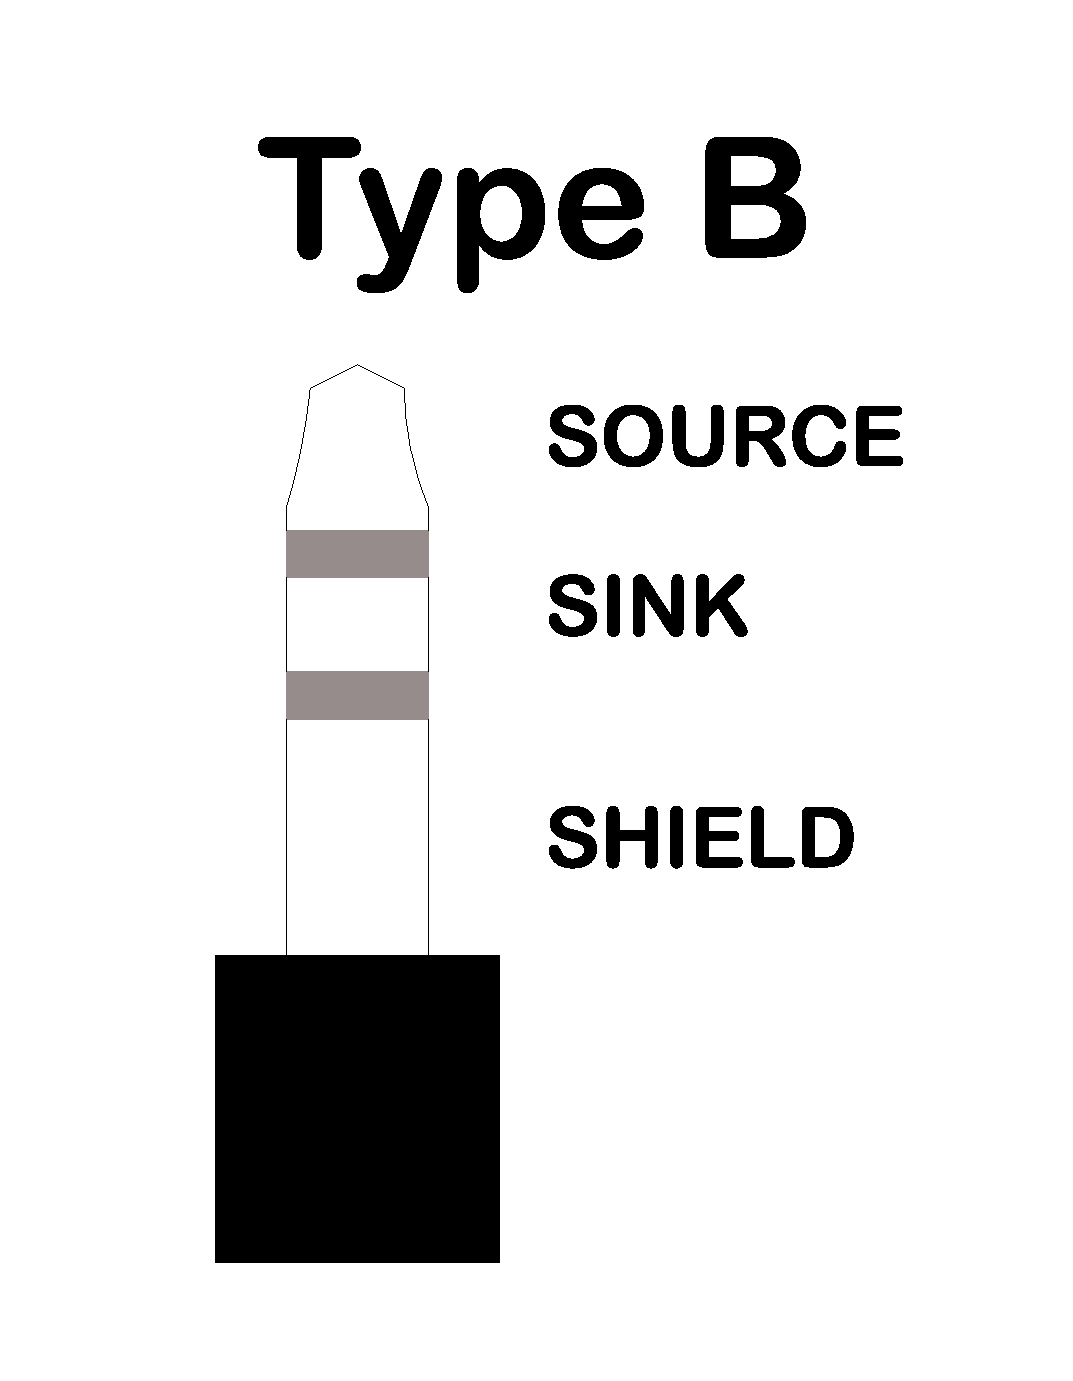
\includegraphics[height=0.3\linewidth]{midi_trs_type_b.eps}
\newline$\bigstar$ Brands using Type B: Arturia, Novation, 1010 Music